%% ============================================================ 51  2023 A-Level P1 Q7
\defQ{51}{}{%
The function f is defined by
\[\mathrm{f}:x\to\left|\frac{2x+4}{3-x}\right|,\qquad x\in\mathbb{R},\qquad x\neq3.\]
\begin{qparts}
\pt{(a)} Sketch the graph of $y=\mathrm{f}(x)$, giving the equations of any asymptotes and the coordinates of the points where the curve meets the axes. \mk{3}
\pt{(b)} Hence state the range of f. \mk{1}
\pt{(c)} Explain why the function $\mathrm{f}^{2}$ does not exist. \mk{1}
\end{qparts}
The domain of f is further restricted to $x\leqslant a$, where $a$ is a constant.
\begin{qparts}
\pt{(d)} State the greatest value of $a$ such that the function $\mathrm{f}^{-1}$ exists. \mk{1}
\pt{(e)} Hence find $\mathrm{f}^{-1}(x)$ and state its domain. \mk{4}
\end{qparts}
\src{2023 A-Level P1 Q7}}
\defS{51}{%
\begin{gtpart}{(a)}{3}\begin{topalign}
y=\left|\frac{2x+4}{3-x}\right|&=\left|-2+\frac{10}{3-x}\right|\\
\text{Asymptotes: }&y=|-2|=2,\quad x=3\\
x=0:\quad y&=\left|\frac43\right|=\frac43\\
y=0:\quad x&=-2
\end{topalign}
\begin{center}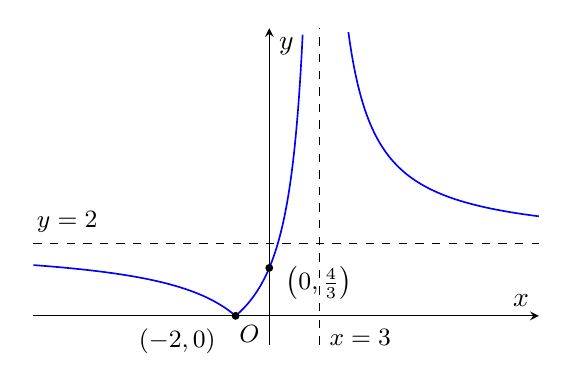
\begin{tikzpicture}
\begin{axis}[width=8cm,height=5.6cm,axis lines=middle,xmin=-14,xmax=16,ymin=-0.8,ymax=8,ticks=none,clip=false,restrict y to domain=-0.8:8,unbounded coords=jump,xlabel=$x$,ylabel=$y$]
\addplot[black,dashed,domain=-14:16]{2};
\addplot[black,dashed] coordinates{(3,-0.8)(3,8)};
\addplot[blue,semithick,domain=-14:2.96,samples=400]{abs((2*x+4)/(3-x))};
\addplot[blue,semithick,domain=3.04:16,samples=400]{abs((2*x+4)/(3-x))};
\addplot[black,only marks,mark=*,mark size=1.2pt] coordinates{(-2,0)(0,1.3333)};
\node[font=\small,anchor=north east] at (axis cs:-2.6,-0.1){$(-2,0)$};
\node[font=\small,anchor=north east] at (axis cs:0,0){$O$};
\node[font=\small,anchor=west] at (axis cs:0.4,0.9){$\left(0,\frac43\right)$};
\node[font=\small,anchor=south] at (axis cs:-12,2.05){$y=2$};
\node[font=\small,anchor=north west] at (axis cs:3,-0.1){$x=3$};
\end{axis}\end{tikzpicture}\end{center}\end{gtpart}
\begin{gtpart}{(b)}{1}\begin{topalign}
\mathrm{R}_{\mathrm f}&=[0,\infty)
\end{topalign}\end{gtpart}
\begin{gtpart}{(c)}{1}\begin{topalign}
\mathrm{R}_{\mathrm f}=[0,\infty),\quad \mathrm{D}_{\mathrm f}&=(-\infty,3)\cup(3,\infty)\\
3\in\mathrm{R}_{\mathrm f},\ 3\notin\mathrm{D}_{\mathrm f}\ &\Rightarrow\ \mathrm{R}_{\mathrm f}\not\subseteq\mathrm{D}_{\mathrm f}\\
\therefore\ \mathrm{f}^{2}&\text{ does not exist}
\end{topalign}\end{gtpart}
\begin{gtpart}{(d)}{1}\begin{topalign}
a&=-2
\end{topalign}
\end{gtpart}
\begin{gtpart}{(e)}{4}\begin{topalign}
x\leqslant-2:\quad\mathrm{f}(x)=\left|\frac{2x+4}{3-x}\right|&=-\frac{2x+4}{3-x}\\
\end{topalign}
\begin{center}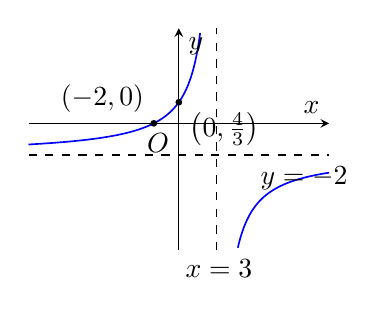
\begin{tikzpicture}[baseline]
\begin{axis}[width=5.4cm,height=4.4cm,axis lines=middle,xmin=-12,xmax=12,ymin=-8,ymax=6,ticks=none,clip=false,restrict y to domain=-8:6,unbounded coords=jump,xlabel=$x$,ylabel=$y$,every node/.append style={font=\scriptsize}]
\addplot[black,dashed] coordinates{(3,-8)(3,6)};
\addplot[black,dashed,domain=-12:12]{-2};
\addplot[blue,semithick,domain=-12:2.9,samples=200]{(2*x+4)/(3-x)};
\addplot[blue,semithick,domain=3.1:12,samples=200]{(2*x+4)/(3-x)};
\addplot[black,only marks,mark=*,mark size=1pt] coordinates{(-2,0)(0,1.333)};
\node[anchor=south east] at (axis cs:-2,0.1){$(-2,0)$};
\node[anchor=north west] at (axis cs:0.1,1.3){$\left(0,\frac43\right)$};
\node[anchor=north east] at (axis cs:0,0){$O$};
\node[anchor=north] at (axis cs:3.2,-8){$x=3$};
\node[anchor=north] at (axis cs:10,-2.1){$y=-2$};
\end{axis}\end{tikzpicture}\quad\raisebox{1.4cm}{$\Longrightarrow$}\quad
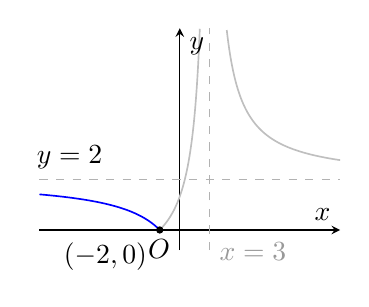
\begin{tikzpicture}[baseline]
\begin{axis}[width=5.4cm,height=4.4cm,axis lines=middle,xmin=-14,xmax=16,ymin=-0.8,ymax=8,ticks=none,clip=false,restrict y to domain=-0.8:8,unbounded coords=jump,xlabel=$x$,ylabel=$y$,every node/.append style={font=\scriptsize}]
\addplot[black!30,dashed,domain=-14:16]{2};
\addplot[black!30,dashed] coordinates{(3,-0.8)(3,8)};
\addplot[black!25,semithick,domain=-2:2.96,samples=300]{abs((2*x+4)/(3-x))};
\addplot[black!25,semithick,domain=3.04:16,samples=300]{abs((2*x+4)/(3-x))};
\addplot[blue,semithick,domain=-14:-2,samples=200]{abs((2*x+4)/(3-x))};
\addplot[black,only marks,mark=*,mark size=1.1pt] coordinates{(-2,0)};
\node[anchor=north east] at (axis cs:-2.3,-0.1){$(-2,0)$};
\node[anchor=north east] at (axis cs:0,0){$O$};
\node[anchor=south] at (axis cs:-11,2.05){$y=2$};
\node[black!40,anchor=north west] at (axis cs:3,-0.1){$x=3$};
\end{axis}\end{tikzpicture}\end{center}
\begin{topalign}
y&=\mathrm{f}(x)\\
-3y+xy&=2x+4\\
x(y-2)&=4+3y\\
x&=\frac{4+3y}{y-2}\\
\mathrm{f}^{-1}(x)&=\frac{4+3x}{x-2},\qquad \mathrm{D}_{\mathrm f^{-1}}=[0,2)
\end{topalign}\end{gtpart}}
%% ============================================================ 52  HCI 2025 Prelim P1 Q8
\defQ{52}{}{%
The function f is defined by
\[\mathrm{f}:x\mapsto\frac{ax-3}{5x-4},\ \text{for }x\in\mathbb{R},\ x\neq\frac45,\ \text{and }a\in\mathbb{R}.\]
\begin{qparts}
\pt{(a)} Find the range of f in terms of $a$. \mk{1}
\end{qparts}
The function f is such that $\mathrm{f}(x)=\mathrm{f}^{-1}(x)$ for all $x$ in the domain of f.
\begin{qparts}
\pt{(b)} Find the value of $a$. \mk{2}
\pt{(c)} Hence find $\mathrm{f}^{2025}(2)$. \mk{2}
\end{qparts}
Another function g is defined by
\[\mathrm{g}:x\mapsto\left(x-\frac15\right)^{2}+\frac25,\ \text{for }x\in\mathbb{R},\ 0<x<\frac35.\]
\begin{qparts}
\pt{(d)} Find the range of fg. \mk{2}
\end{qparts}
\src{HCI 2025 Prelim P1 Q8}}
\defS{52}{%
\begin{gtpart}{(a)}{1}\begin{topalign}
\text{Horizontal asymptote: }y&=\frac a5\\
\mathrm{R}_{\mathrm f}&=\mathbb{R}\setminus\left\{\frac a5\right\}
\end{topalign}\end{gtpart}
\begin{gtpart}{(b)}{2}\begin{topalign}
y&=\frac{ax-3}{5x-4}\\
5xy-4y&=ax-3\\
5xy-ax&=4y-3\\
x&=\frac{4y-3}{5y-a}\\
\mathrm{f}^{-1}(x)&=\frac{4x-3}{5x-a},\quad x\in\mathbb{R},\ x\neq\frac a5\\
\mathrm{f}(x)=\mathrm{f}^{-1}(x)\ &\Rightarrow\ a=4
\end{topalign}\end{gtpart}
\begin{gtpart}{(c)}{2}\begin{topalign}
\mathrm{f}^{-1}(x)=\mathrm{f}(x)\ &\Rightarrow\ \mathrm{f}^{2}(x)=\mathrm{f}\mathrm{f}^{-1}(x)=x\\
\mathrm{f}^{2025}(2)&=\mathrm{f}^{2}\big(\mathrm{f}^{2023}(2)\big)\\
&=\mathrm{f}^{2}\big(\mathrm{f}^{2021}(2)\big)\\
&=\cdots\\
&=\mathrm{f}(2)\\
&=\frac{4(2)-3}{5(2)-4}=\frac56
\end{topalign}\end{gtpart}
\begin{gtpart}{(d)}{2}\begin{topalign}
\mathrm{R}_{\mathrm g}&=\left[\frac25,\frac{14}{25}\right)\\
\mathrm{f}(x)&=\frac{4x-3}{5x-4}\\
\left(0,\frac35\right)\xrightarrow{\ \mathrm g\ }\left[\frac25,\frac{14}{25}\right)&\xrightarrow{\ \mathrm f\ }\left(\frac{19}{30},\frac7{10}\right]\\
\mathrm{R}_{\mathrm{fg}}&=\left(\frac{19}{30},\frac7{10}\right]
\end{topalign}
\begin{center}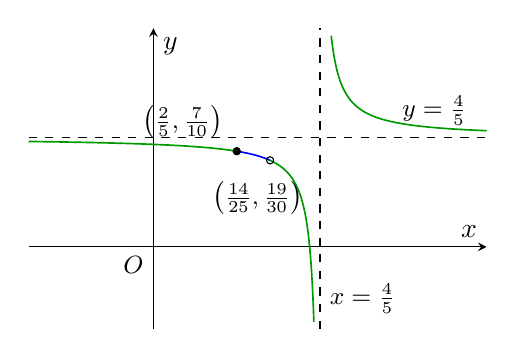
\begin{tikzpicture}
\begin{axis}[width=7.4cm,height=5.4cm,axis lines=middle,xmin=-0.6,xmax=1.6,ymin=-0.6,ymax=1.6,ticks=none,clip=false,restrict y to domain=-0.6:1.6,unbounded coords=jump,xlabel=$x$,ylabel=$y$]
\addplot[black,dashed,domain=-0.6:1.6]{0.8};
\addplot[black,dashed] coordinates{(0.8,-0.6)(0.8,1.6)};
\addplot[green!60!black,semithick,domain=-0.6:0.4,samples=100]{(4*x-3)/(5*x-4)};
\addplot[green!60!black,semithick,domain=0.56:0.79,samples=200]{(4*x-3)/(5*x-4)};
\addplot[green!60!black,semithick,domain=0.81:1.6,samples=200]{(4*x-3)/(5*x-4)};
\addplot[blue,semithick,domain=0.4:0.56,samples=60]{(4*x-3)/(5*x-4)};
\addplot[black,only marks,mark=*,mark size=1.3pt] coordinates{(0.4,0.7)};
\addplot[black,only marks,mark=o,mark size=1.3pt,fill=white] coordinates{(0.56,0.6333)};
\node[font=\small,anchor=north east] at (axis cs:0,0){$O$};
\node[font=\small,anchor=south east] at (axis cs:0.38,0.72){$\left(\frac25,\frac7{10}\right)$};
\node[font=\small,anchor=north] at (axis cs:0.5,0.55){$\left(\frac{14}{25},\frac{19}{30}\right)$};
\node[font=\small,anchor=south] at (axis cs:1.35,0.82){$y=\frac45$};
\node[font=\small,anchor=north west] at (axis cs:0.8,-0.2){$x=\frac45$};
\end{axis}\end{tikzpicture}\end{center}\end{gtpart}}
%% ============================================================ 53  VJC 2025 Prelim P1 Q5(a), (b)
\defQ{53}{}{%
The function f is given by
\[\mathrm{f}(x)=\begin{cases}2+\sqrt{2^{2}-(x-2)^{2}}, & 0<x\leqslant4,\\[1ex] 2-\sqrt{2^{2}-(x-6)^{2}}, & 4<x\leqslant8.\end{cases}\]
It is given that $\mathrm{f}(x)=\mathrm{f}(x+8)$ for all real values of $x$.
\begin{qparts}
\pt{(a)} On the diagram in the Printed Answer Book, sketch the graph of $y=\mathrm{f}(x)$ for $-6\leqslant x\leqslant7$, indicating clearly the coordinates of the end points and the points where the graph cuts the axes. \mk{3}
\pt{(b)} Without integrating, write down the exact area of the region bounded by $y=\mathrm{f}(x)$, the line $x=4$, the $x$-axis and the $y$-axis. \mk{1}
\end{qparts}
\src{VJC 2025 Prelim P1 Q5(a), (b)}}
\defS{53}{%
\begin{gtpart}{(a)}{3}{\color{gray}\small
\begin{minipage}[t]{0.48\linewidth}\centering
$\begin{aligned}y&=2+\sqrt{2^{2}-(x-2)^{2}}\\ y-2&=\sqrt{2^{2}-(x-2)^{2}}\\ (x-2)^{2}+(y-2)^{2}&=2^{2}\end{aligned}$\par
Centre $(2,2)$, radius 2.\par
Since it is a positive square root, it is the top half of this circle.
\end{minipage}\hfill
\begin{minipage}[t]{0.48\linewidth}\centering
$\begin{aligned}y&=2-\sqrt{2^{2}-(x-6)^{2}}\\ y-2&=-\sqrt{2^{2}-(x-6)^{2}}\\ (x-6)^{2}+(y-2)^{2}&=2^{2}\end{aligned}$\par
Centre $(6,2)$, radius 2.\par
Since it is a negative square root, it is the bottom half of this circle.
\end{minipage}\par}\vspace{-2mm}
\begin{center}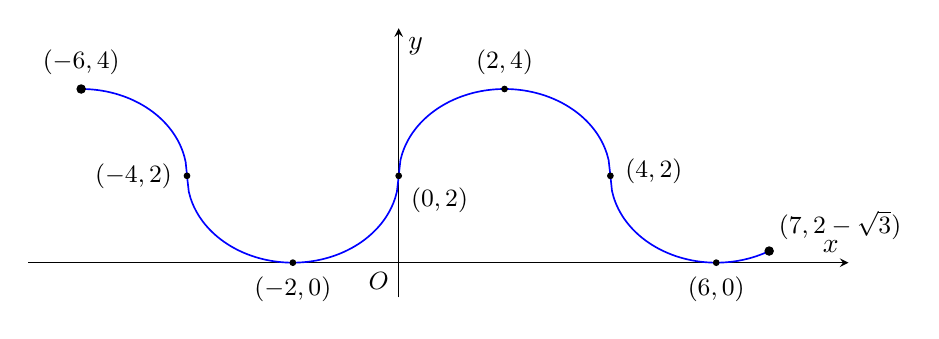
\begin{tikzpicture}
\begin{axis}[width=12cm,height=5cm,axis lines=middle,xmin=-7,xmax=8.5,ymin=-0.8,ymax=5.4,ticks=none,clip=false,restrict y to domain=-0.8:5.4,unbounded coords=jump,xlabel=$x$,ylabel=$y$]
\addplot[blue,semithick,domain=-6:-4,samples=80]{2+sqrt(max(0,4-(x+6)^2))};
\addplot[blue,semithick,domain=-4:0,samples=120]{2-sqrt(max(0,4-(x+2)^2))};
\addplot[blue,semithick,domain=0:4,samples=120]{2+sqrt(max(0,4-(x-2)^2))};
\addplot[blue,semithick,domain=4:7,samples=100]{2-sqrt(max(0,4-(x-6)^2))};
\addplot[black,only marks,mark=*,mark size=1.5pt] coordinates{(-6,4)(7,0.268)};
\addplot[black,only marks,mark=*,mark size=1pt] coordinates{(-4,2)(-2,0)(0,2)(2,4)(4,2)(6,0)};
\node[font=\small,anchor=south] at (axis cs:-6,4.1){$(-6,4)$};
\node[font=\small,anchor=east] at (axis cs:-4.1,2){$(-4,2)$};
\node[font=\small,anchor=north] at (axis cs:-2,-0.1){$(-2,0)$};
\node[font=\small,anchor=north west] at (axis cs:0.05,1.95){$(0,2)$};
\node[font=\small,anchor=south] at (axis cs:2,4.1){$(2,4)$};
\node[font=\small,anchor=west] at (axis cs:4.1,2.1){$(4,2)$};
\node[font=\small,anchor=north] at (axis cs:6,-0.1){$(6,0)$};
\node[font=\small,anchor=south west] at (axis cs:7,0.3){$(7,2-\sqrt3)$};
\node[font=\small,anchor=north east] at (axis cs:0,0){$O$};
\end{axis}\end{tikzpicture}\end{center}\end{gtpart}
\begin{gtpart}{(b)}{1}\begin{topalign}
\text{Area}&=2\times4+\frac12\pi\left(2^{2}\right)=8+2\pi
\end{topalign}\end{gtpart}}
%% ============================================================ 54  HCI 2024 Promo Q8
\defQ{54}{}{%
The function f is defined by
\[\mathrm{f}(x)=\begin{cases}2-\ln(x+\mathrm{e}) & \text{for }-\mathrm{e}<x<0,\\[1ex] \cos\left(\dfrac{\pi}{2}x\right) & \text{for }0\leqslant x\leqslant1.\end{cases}\]
\begin{qparts}
\pt{(a)} Given that the inverse function $\mathrm{f}^{-1}$ exists, find the exact value of $m$ if $\mathrm{f}^{-1}(m)=-1$. \mk{2}
\end{qparts}
Another function g is defined by
\[\mathrm{g}(x)=\sin x,\qquad\text{for }0\leqslant x\leqslant\frac{\pi}{4}.\]
\begin{qparts}
\pt{(b)} Explain why the composite function fg exists. \mk{2}
\pt{(c)} Find the exact value of $\mathrm{fg}\left(\dfrac{\pi}{6}\right)$. \mk{2}
\end{qparts}
The domain of f is further restricted to $0\leqslant x\leqslant1$.
\begin{qparts}
\pt{(d)} By considering $\mathrm{f}^{2}(1)$ and $\mathrm{f}^{3}(1)$, deduce the value(s) of $\mathrm{f}^{n}(1)$ where $n$ is a positive integer. \mk{2}
\end{qparts}
\src{HCI 2024 Promo Q8}}
\defS{54}{%
\begin{gtpart}{(a)}{2}\begin{topalign}
\mathrm{f}^{-1}(m)&=-1\\
m&=\mathrm{f}(-1)\\
&=2-\ln(\mathrm{e}-1)
\end{topalign}\end{gtpart}
\begin{gtpart}{(b)}{2}\begin{topalign}
\mathrm{R}_{\mathrm g}&=\left[0,\frac{1}{\sqrt2}\right]\\
\mathrm{D}_{\mathrm f}&=(-\mathrm{e},1]\\
\mathrm{R}_{\mathrm g}\subseteq\mathrm{D}_{\mathrm f}\ &\Rightarrow\ \mathrm{fg}\text{ exists}
\end{topalign}\end{gtpart}
\begin{gtpart}{(c)}{2}\begin{topalign}
\mathrm{fg}\left(\frac{\pi}{6}\right)&=\mathrm{f}\left(\frac12\right)\\
&=\cos\left(\frac{\pi}{4}\right)\\
&=\frac{1}{\sqrt2}
\end{topalign}\end{gtpart}
\begin{gtpart}{(d)}{2}
\begin{center}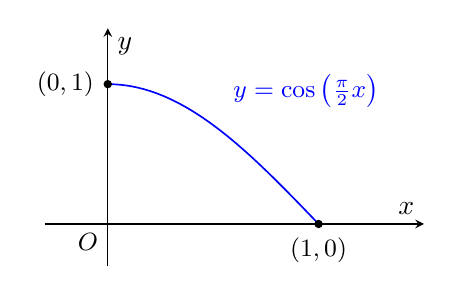
\begin{tikzpicture}
\begin{axis}[width=6.4cm,height=4.6cm,axis lines=middle,xmin=-0.3,xmax=1.5,ymin=-0.3,ymax=1.4,ticks=none,clip=false,restrict y to domain=-0.3:1.4,unbounded coords=jump,xlabel=$x$,ylabel=$y$]
\addplot[blue,semithick,domain=0:1,samples=80]{cos(deg(pi*x/2))};
\addplot[black,only marks,mark=*,mark size=1.3pt] coordinates{(0,1)(1,0)};
\node[font=\small,anchor=east] at (axis cs:-0.02,1){$(0,1)$};
\node[font=\small,anchor=north] at (axis cs:1,-0.03){$(1,0)$};
\node[font=\small,anchor=north east] at (axis cs:0,0){$O$};
\node[font=\small,blue,anchor=west] at (axis cs:0.55,0.95){$y=\cos\left(\frac{\pi}{2}x\right)$};
\end{axis}\end{tikzpicture}\end{center}
\begin{topalign}
\mathrm{f}^{2}(1)&=\mathrm{f}\big[\mathrm{f}(1)\big]=\mathrm{f}(0)=1\\
\mathrm{f}^{3}(1)&=\mathrm{f}\big[\mathrm{f}^{2}(1)\big]=\mathrm{f}(1)=0\\
\mathrm{f}^{n}(1)&=\begin{cases}0 & \text{if $n$ is odd}\\ 1 & \text{if $n$ is even}\end{cases}
\end{topalign}\end{gtpart}}
%% ============================================================ 55  ACJC 2022 Prelim P2 Q1
\defQ{55}{}{%
The function f is defined by
\[\mathrm{f}(x)=1-ax,\ x\in\mathbb{R},\ \text{where $a$ is a real constant.}\]
The function g is defined by
\[\mathrm{g}(x)=\begin{cases}x^{2}+3 & \text{for}\quad 0\leqslant x\leqslant2,\\ 7-x & \text{for}\quad 2<x\leqslant7.\end{cases}\]
\begin{qparts}
\pt{(i)} Find the set of possible values of $a$ such that $\mathrm{f}^{-1}$ exist. \mk{1}
\pt{(ii)} If $a=2$, describe a sequence of transformations that transform the graph of $y=\mathrm{g}(x)$ onto the graph of $y=\mathrm{fg}(x)$. \mk{3}
\pt{(iii)} The function gg is defined by
\[\mathrm{gg}(x)=\begin{cases}\mathrm{h}_1(x) & \text{for}\quad 0\leqslant x\leqslant2,\\ \mathrm{h}_2(x) & \text{for}\quad 2<x<5,\\ \mathrm{h}_3(x) & \text{for}\quad 5\leqslant x\leqslant7.\end{cases}\]
Find $\mathrm{h}_1(x)$, $\mathrm{h}_2(x)$ and $\mathrm{h}_3(x)$. \mk{3}
\end{qparts}
\src{ACJC 2022 Prelim P2 Q1}}
\defS{55}{%
\begin{gtpart}{(i)}{1}\begin{topalign}
a&\in\mathbb{R}\setminus\{0\}
\end{topalign}\end{gtpart}
\begin{gtpart}{(ii)}{3}\begin{topalign}
y=\mathrm{fg}(x)&=1-2\mathrm{g}(x)
\end{topalign}
Reflection of the graph of $y=\mathrm{g}(x)$ in the $x$-axis, followed by scaling by scale factor 2 parallel to the $y$-axis, followed by translation 1 unit in the positive $y$-direction.\par
\textbf{OR}\par
Translation of the graph of $y=\mathrm{g}(x)$ by $\frac12$ unit in the negative $y$-direction followed by reflection in the $x$-axis followed by scaling by scale factor 2 parallel to the $y$-axis.\par
\textbf{OR}\par
Translation of the graph of $y=\mathrm{g}(x)$ by $\frac12$ unit in the negative $y$-direction followed by scaling by scale factor 2 parallel to the $y$-axis followed by reflection in the $x$-axis.
\end{gtpart}
\begin{gtpart}{(iii)}{3}\begin{topalign}
\mathrm{gg}(x)&=\begin{cases}7-\left(x^{2}+3\right) & \text{for}\quad 0\leqslant x\leqslant2\\ 7-(7-x) & \text{for}\quad 2<x<5\\ (7-x)^{2}+3 & \text{for}\quad 5\leqslant x\leqslant7\end{cases}\\[1ex]
\therefore\ \mathrm{gg}(x)&=\begin{cases}4-x^{2} & \text{for}\quad 0\leqslant x\leqslant2\\ x & \text{for}\quad 2<x<5\\ x^{2}-14x+52 & \text{for}\quad 5\leqslant x\leqslant7\end{cases}
\end{topalign}\end{gtpart}}
%% ============================================================ 56  CJC 2025 Prelim P2 Q2(a), (b)
\defQ{56}{}{%
Functions f and g are defined by
\[\mathrm{f}:x\to\frac{4}{(x-4)^{2}},\quad x\in\mathbb{R},\ x\neq4,\]
\[\mathrm{g}:x\to\ln\left(1+\frac1x\right),\quad x\in\mathbb{R},\ x>0.\]
\begin{qparts}
\pt{(a)} Sketch the graph of $y=\mathrm{f}(x)$, stating the equations of any asymptotes, the coordinates of the points where it crosses the axes and the coordinates of the turning points, if any. \mk{2}
\pt{(b)} Show that gf exists. Hence find the rule, domain and range of gf. \mk{4}
\end{qparts}
\src{CJC 2025 Prelim P2 Q2(a), (b)}}
\defS{56}{%
\begin{gtpart}{(a)}{2}
\begin{center}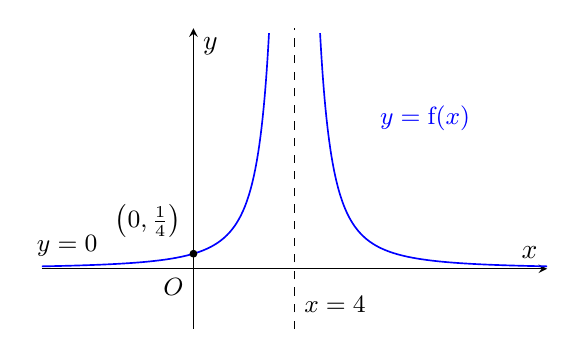
\begin{tikzpicture}
\begin{axis}[width=8cm,height=5.4cm,axis lines=middle,xmin=-6,xmax=14,ymin=-1,ymax=4,ticks=none,clip=false,restrict y to domain=-1:4,unbounded coords=jump,xlabel=$x$,ylabel=$y$]
\addplot[black,dashed] coordinates{(4,-1)(4,4)};
\addplot[blue,semithick,domain=-6:3.02,samples=300]{4/(x-4)^2};
\addplot[blue,semithick,domain=4.98:14,samples=300]{4/(x-4)^2};
\addplot[black,only marks,mark=*,mark size=1.2pt] coordinates{(0,0.25)};
\node[font=\small,anchor=south east] at (axis cs:-0.1,0.35){$\left(0,\frac14\right)$};
\node[font=\small,anchor=north east] at (axis cs:0,0){$O$};
\node[font=\small,anchor=south] at (axis cs:-5,0.05){$y=0$};
\node[font=\small,anchor=north west] at (axis cs:4,-0.3){$x=4$};
\node[font=\small,blue,anchor=west] at (axis cs:7,2.5){$y=\mathrm{f}(x)$};
\end{axis}\end{tikzpicture}\end{center}\end{gtpart}
\begin{gtpart}{(b)}{4}
For gf to exist, $\mathrm{R}_{\mathrm f}\subseteq\mathrm{D}_{\mathrm g}$,
\begin{topalign}
\mathrm{R}_{\mathrm f}&=(0,\infty)\\
\mathrm{D}_{\mathrm g}&=(0,\infty)
\end{topalign}
Since $\mathrm{R}_{\mathrm f}\subseteq\mathrm{D}_{\mathrm g}$, gf exists (shown)
\begin{topalign}
\mathrm{gf}(x)&=\mathrm{g}\left[\frac{4}{(x-4)^{2}}\right]\\
&=\ln\left[1+\left(\frac{1}{\frac{4}{(x-4)^{2}}}\right)\right]\\
&=\ln\left[1+\frac{(x-4)^{2}}{4}\right]\\
\mathrm{D}_{\mathrm{gf}}=\mathrm{D}_{\mathrm f}&=(-\infty,4)\cup(4,\infty)
\end{topalign}
OR
\begin{topalign}
\mathrm{D}_{\mathrm{gf}}=\mathrm{D}_{\mathrm f}&=\mathbb{R}\setminus\{4\}
\end{topalign}
\textbf{\underline{Method 1: Mapping}}
\[\mathrm{D}_{\mathrm f}=(-\infty,4)\cup(4,\infty)\xrightarrow{\ \mathrm f\ }\mathrm{R}_{\mathrm f}=(0,\infty)\xrightarrow{\ \mathrm g\ }\mathrm{R}_{\mathrm{gf}}=(0,\infty)\]
\begin{center}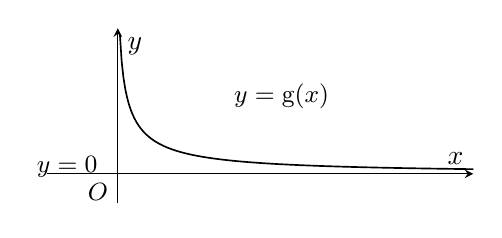
\begin{tikzpicture}
\begin{axis}[width=7cm,height=3.8cm,axis lines=middle,xmin=-2,xmax=10,ymin=-0.6,ymax=3,ticks=none,clip=false,xlabel=$x$,ylabel=$y$,restrict y to domain=-0.6:3]
\addplot[black,semithick,domain=0.06:10,samples=200]{ln(1+1/x)};
\node[font=\small,anchor=north east] at (axis cs:0,0){$O$};
\node[font=\small,anchor=east] at (axis cs:-0.3,0.15){$y=0$};
\node[font=\small,anchor=west] at (axis cs:3,1.6){$y=\mathrm{g}(x)$};
\end{axis}\end{tikzpicture}\end{center}
\textbf{\underline{Method 2: Sketch $y=\mathrm{gf}(x)$ for given domain}}
\begin{center}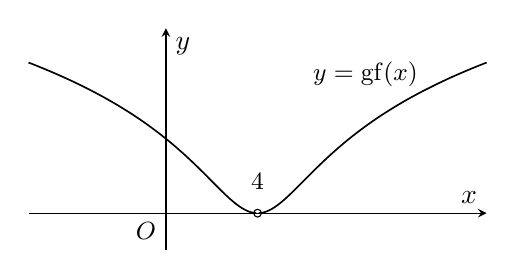
\begin{tikzpicture}
\begin{axis}[width=7.4cm,height=4.4cm,axis lines=middle,xmin=-6,xmax=14,ymin=-0.8,ymax=4,ticks=none,clip=false,xlabel=$x$,ylabel=$y$]
\addplot[black,semithick,domain=-6:3.95,samples=200]{ln(1+(x-4)^2/4)};
\addplot[black,semithick,domain=4.05:14,samples=200]{ln(1+(x-4)^2/4)};
\addplot[black,only marks,mark=o,mark size=1.4pt,fill=white] coordinates{(4,0)};
\node[font=\small,anchor=south] at (axis cs:4,0.3){$4$};
\node[font=\small,anchor=north east] at (axis cs:0,0){$O$};
\node[font=\small,anchor=west] at (axis cs:6,3){$y=\mathrm{gf}(x)$};
\end{axis}\end{tikzpicture}\end{center}
\begin{topalign}
\mathrm{R}_{\mathrm{gf}}&=(0,\infty)
\end{topalign}
\end{gtpart}}
%% ============================================================ 57  2016 A-Level P1 Q10(b)
\defQ{57}{}{%
\fhlp{The function $\mathrm{g}$, with domain the set of non-negative integers, is given by
\[\mathrm{g}(n)=\begin{cases}1&\text{for }n=0,\\2+\mathrm{g}\left(\tfrac12n\right)&\text{for }n\text{ even},\\1+\mathrm{g}(n-1)&\text{for }n\text{ odd}.\end{cases}\]}
\begin{qparts}
\pt{(i)} \fhl{Find $\mathrm{g}(4)$, $\mathrm{g}(7)$ and $\mathrm{g}(12)$.} \mk{\fhl{3}}
\pt{(ii)} Does $\mathrm{g}$ have an inverse? Justify your answer. \mk{\fhl{2}}
\end{qparts}
\src{2016 A-Level P1 Q10(b)}}
\defS{57}{%
\begin{gtpart}{(i)}{3}\fhlp{$\begin{aligned}[t]
\mathrm{g}(4)&=2+\mathrm{g}\left(\tfrac12\times4\right)=2+\mathrm{g}(2)=2+\left[2+\mathrm{g}\left(\tfrac12\times2\right)\right]=4+\mathrm{g}(1)\\
&=4+\left[1+\mathrm{g}(1-1)\right]=5+\mathrm{g}(0)=5+1=6\\[1ex]
\mathrm{g}(7)&=1+\mathrm{g}(7-1)=1+\mathrm{g}(6)=1+\left[2+\mathrm{g}\left(\tfrac12\times6\right)\right]=3+\mathrm{g}(3)\\
&=3+\left[1+\mathrm{g}(3-1)\right]=4+\mathrm{g}(2)=4+\left[2+\mathrm{g}\left(\tfrac12\times2\right)\right]=6+\mathrm{g}(1)\\
&=6+\left[1+\mathrm{g}(1-1)\right]=7+\mathrm{g}(0)=7+1=8\\[1ex]
\mathrm{g}(12)&=2+\mathrm{g}\left(\tfrac12\times12\right)=2+\mathrm{g}(6)=2+\left[2+\mathrm{g}\left(\tfrac12\times6\right)\right]=4+\mathrm{g}(3)\\
&=4+\left[1+\mathrm{g}(3-1)\right]=5+\mathrm{g}(2)=5+\left[2+\mathrm{g}\left(\tfrac12\times2\right)\right]=7+\mathrm{g}(1)\\
&=7+\left[1+\mathrm{g}(1-1)\right]=8+\mathrm{g}(0)=8+1=9
\end{aligned}$}\par\smallskip
\fhl{{\footnotesize Solution source: Achevas (Jack Ng), ``A-Level H2 Maths 2016 -- Paper 1'', www.achevas.com.}}\end{gtpart}
\begin{gtpart}{(ii)}{2}\fhlp{$\begin{aligned}[t]
\mathrm{g}(5)&=1+\mathrm{g}(4)=1+6=7\\
\mathrm{g}(6)&=2+\mathrm{g}(3)=2+\left[1+\mathrm{g}(2)\right]=3+\mathrm{g}(2)\\
&=3+\left[2+\mathrm{g}(1)\right]=5+\mathrm{g}(1)=5+\left[1+\mathrm{g}(0)\right]=6+1=7
\end{aligned}$}\par\smallskip
\fhl{Since $\mathrm{g}(5)=\mathrm{g}(6)$, $\mathrm{g}$ does not have an inverse.}\end{gtpart}}
